\documentclass[twocolumn]{article}
\usepackage{graphicx}
\usepackage{amsmath,amssymb}
\usepackage[numbers]{natbib} % optional
\usepackage{booktabs}
\usepackage{csquotes}
\usepackage{afterpage}

\title{Interpretable Deep Learning for Robust Drug Mechanism Prediction \\ in High-Throughput Gene Expression Data}
\author{Navinda Hewawickrama \& Sugandima Vidanagamachchi}
\date{April 2025}
\begin{document}
\onecolumn
\maketitle
\begin{abstract}
        The LINCS L1000 dataset, a massive library of how human cells react to different drugs, holds immense promise for understanding and treating diseases. It offers a powerful resource for discovering a drug's true mechanism of action (MoA), but getting to those answers isn't straightforward. Scientists using this data must overcome major computational hurdles, including its sheer size, inherent experimental noise, and incomplete information.To understand how the research community is tackling these problems, we took a deep dive into the last decade of scientific literature. We systematically reviewed 28 key studies published between 2014 and 2025 that use machine learning and deep learning to unlock the secrets hidden within the L1000 dataset, aiming to find new uses for existing drugs and identify novel therapeutic targets.Our review uncovered a fascinating story of technological evolution. We saw a clear shift from traditional machine learning methods to more powerful deep learning models that could better handle the data's complexity. As researchers built more sophisticated models using tools like Graph Neural Networks, their predictive accuracy improved. However, a crucial challenge remains: making these powerful \enquote{black box} models understandable. This has sparked an important new trend toward \enquote{explainable AI} (XAI)—a push to not only get the right answer but to understand why it's the right answer.So, what does this all mean? Our work shows that the field is at a crossroads, moving beyond simply predicting a drug's effect to truly understanding the mechanism behind it. The next great leap forward will come from building models that are not only accurate but also trustworthy and transparent. By developing smarter, more interpretable frameworks and combining different types of data, we can finally bridge the gap from massive datasets to real-world impact, turning this wealth of information into new medicines and better treatments for patients.
\end{abstract}

\twocolumn
\section{Introduction}
\subsection{Rationale}
The search for new therapeutics depends a lot on understanding how drugs interact with biological systems. High-throughput platforms, such as The Cancer Dependency Map (DepMap) for genetic vulnerabilities, The Genotype-Tissue Expression (GTEx) project for baseline tissue-specific gene expression, The Human Protein Atlas (HPA), the Library of Integrated Network-Based Cellular Signatures (LINCS) L1000 for transcriptomic responses to chemicals, etc\. have transformed pharmacogenomics by providing large-scale datasets on gene expression responses to multiple chemical perturbations. The LINCS project, specifically, profiles responses to about 20,000 compounds across numerous human cell lines, uniquely inferring approximately 82\% of the transcriptome from just 978 landmark genes to achieve massive scale and cost-efficiency\cite{subramanian2017next,mcdermott2019deep}.

Despite its transformative potential, the LINCS L1000 platform presents several inherited challenges. These include the high dimensionality of the data and systemic noise from the experimental setup, like the use of computational predictions and technical inconsistencies in the assay process. Furthermore, incomplete or inconsistent metadata (e.g., dosage, exposure time) can significantly affect reproducibility and model accuracy\cite{stathias2018sustainable}. The complexity of accurately interpreting drug mechanisms of action (MoAs) from these vast and noisy transcriptional responses remains a huge hurdle. While earlier studies have utilized LINCS data for MoA prediction\cite{everett2023combining,gao2022deep,el2017integrative,wang2016drug,subramanian2017next,wu2022deep,liao2023open}, traditional machine learning methods such as Support Vector Machines (SVM), k-Nearest Neighbours (KNN), and Random Forests have often struggled with the high dimensionality and non-linear relationships in the data, limiting their predictive accuracy and scalability\cite{li2020deep,everett2023combining}.

Even though there is progress, critical gaps still remain. One key limitation is that data quality issues, including metadata incompleteness and inherent experimental noise, are often treated as a minor preprocessing step rather than the main factor that determines the model accuracy and interoperability\cite{stathias2018sustainable}. Additionally, there are limited studies into how deep learning and knowledge graph approaches can be used to integrate LINCS data with external biological networks. Also, a few studies have shown whether such integrated, explainable approaches can achieve a balance between robustness, accuracy, and cross-system interoperability in MoA prediction\cite{ye2025knowledge,evangelista2023toxicology,wu2022deep}. This study addresses these gaps by systematically reviewing the current computational methods, giving special attention to how they handle data quality, combining multimodal knowledge, and pursuing the ultimate goal of achieving reliable and interpretable results.

\subsection{Objectives}
This systematic literature review aims to integrate and evaluate critically the current research on the use of LINCS L1000 data for predicting drug mechanisms of action. It focuses on identifying methods used to handle the inherent inconsistencies and missing metadata challenges, evaluating their effectiveness, and highlighting unresolved challenges and opportunities for methodological improvement. Specifically, this systematic review tries to answer the following research questions.
\begin{itemize}  
  \item \textbf{R1:} What techniques have been used to predict drug mechanisms of action from LINCS gene expression data, and how do they balance accuracy, scalability, and interpretability, in high-dimensional biomedical contexts?
  \item \textbf{R2:} How do data quality issues (e.g., noise, inconsistencies) affect the performance and generalizability of predictive models, and what computational methods have been used to address these challenges?
  \item \textbf{R3:} Are there frameworks that effectively integrate external knowledge (e.g., drug structures, biological networks) with transcriptomic data, and how do they impact model interpretability, generalizability, and explainability?
\end{itemize}
By addressing these questions, the review aims to look into the development of more robust, interpretable, and effective analytical frameworks for MoA prediction based on the LINCS L1000-like high-throughput gene expression datasets.

\subsection{Road Map}
The article is divided into sections, which will help us understand the process. Section 2 will provide the methodology, where details about how studies for the literature review was selected, how they were filtered, what the selection process was, how data were collected, etc., will be explained in detail. In section 3, the results of the Methods section will be explained in detail, explaining the results of the search criteria, which studies were selected, the results of the selected studies, etc.. Section 4 will provide the details of the discussion of the found evidence. Section 5 will hold the details of the other information, such as limitations, other information, conflicts of interest, future works, etc.
\section{Methods}
The Preferred Reporting Items for Systematic Reviews and Meta-Analyses (PRISMA) guidelines were followed to produce a systematic review\cite{page2021prisma}.\linebreak PRISMA is a standard methodology that maintains and ensures a certain level of quality in the review process. The review protocol was developed by defining the article selection criteria, search strategy, data extraction, and data analysis procedures.
\subsection{Eligibility Criteria}\label{subsec:Eligibility Criteria}
Based on the search strategy, an initial screening of study titles and abstracts was performed to identify articles that focus on LINCS L1000 data analytics, drug mechanism prediction, and methods for handling data quality issues in genomic or biomedical contexts. Articles that met the following criteria were included for study selection: 
\\
\textbf{Topic: }Focused on mechanisms of action (MoA) prediction, target identification, or related pharmacogenomic tasks like drug repurposing and toxicity screening using LINCS L1000 gene expression data.
\\
\textbf{Approach: }Using computational methods (e.g., machine learning, deep learning, or knowledge graph integration) for analyzing LINCS L1000 data or integrating it with other biological datasets. This includes studies that propose or apply explainable AI (XAI) or other techniques to enhance model interpretability.
\\
\textbf{Data Challenges: }Discussed or addressed challenges related to data quality, such as label noise, metadata incompleteness or inconsistencies, systemic noise from the experimental setup, such as technical artifacts, the computational inference of the non-landmark genes or high dimensionality.
\\
\textbf{Publication Year: }Studies published between 2014 and 2025 to capture the evolution of methods following the major LINCS data releases.
\\
Focused mainly on the work that used the LINCS L1000 data set. 
\subsection{Information Sources}
The following electronic databases were searched for information sources.
\begin{itemize}
    \item PubMed
    \item Google Scholar
    \item arXiv
    \item IEEE
    \item Other (Research Gate, NIH, Springer)
\end{itemize}

\subsection{Search Strategy}
The search was constructed using a combination of keywords related to the core components of the research, using Boolean operators (AND, OR) to broaden or refine the search. Key search terms included words regarding
\\
\begin{itemize}
    \item \textbf{Core Data:} `LINCS L1000', `Connectivity Map', `gene expression',`transcriptomic'.
    \item  \textbf{Task to do:} `drug mechanism of action', `drug mechanism prediction', `pharmacogenomics', `drug response', `MoA prediction'
    \item  \textbf{Methods:} `machine learning', `deep learning', predictive models', `explainable AI', `neural networks', `graph neural networks'
    \item  \textbf{Challenges:} `metadata incompleteness',`missing data imputation', `deep learning imputation', `data inconsistencies'
    \item  \textbf{Data integration:} `knowledge graph', `multi-source integration', `multimodal fusion'
\end{itemize}
A sample search string used in PubMed was\\
\\
(`LINCS L1000' OR `Library of Integrated Network-Based Cellular Signature') AND 
(`drug mechanism' OR `mechanism of action' OR `MoA prediction') AND 
(`gene expression' OR `pharmacogenomics') AND 
(`machine learning' OR `deep learning' OR `knowledge graph') AND 
(`metadata' OR `missing data' OR `data integration')
\\
Search strategies were adapted for each database as appropriate.
Search strings used to search relevant papers.
\begin{enumerate}
    \item \textbf{Broad Search for Core Methods:} This string is designed to find the most common papers that apply machine learning or deep learning to LINCS L1000 for MoA prediction.
    (`LINCS L1000' OR `Connectivity Map') AND (`drug mechanism of action' OR `MoA prediction') AND (`machine learning' OR `deep learning')
    \item \textbf{Focused Search on Data Quality Challenges:} This string specifically targets papers that discuss the challenges of data quality, noise, or metadata, which is central to R2.
    (`LINCS L1000' OR `transcriptomic') AND (`drug response' OR `pharmacogenomics') AND (`metadata incompleteness' OR `data inconsistencies' OR `missing data imputation')
    \item \textbf{Focused Search on Explainable AI (XAI) and Integration:} This string is tailored to find advanced papers that integrate external knowledge using knowledge graphs or focus on interpretability, which is key to R3.
    (`LINCS L1000') AND (`mechanism of action' OR `MoA prediction') AND (`knowledge graph' OR `explainable AI' OR `multimodal fusion')
    \item \textbf{Search for Advanced Deep Learning Architectures:} This string hones in on the cutting-edge models you discuss in your results, like GNNs and Transformers, to ensure you capture the latest methodological advancements.
    (`LINCS L1000' OR `gene expression') AND (`drug mechanism prediction') AND (`graph neural networks' OR `transformer' OR `attention mechanism')
\end{enumerate}

\subsection{Selection Process}
The study selection process was done guided by the PRISMA method, beginning with a thorough search across the specified databases.
\\
\subsubsection{Initial Screening (Title and Abstract)}
All records identified from the electronic databases were imported into a reference management tool (Mendeley) to manage them according to their relevance and to remove duplicates. After removing the duplicates, the rest of the records were screened by the title and the abstracts against the predefined eligibility criteria mention in\ref{subsec:Eligibility Criteria}. Any article that fit the eligibility criteria was advanced to the full-text review stage. The reason for exclusion at this stage is based on the relevance of the content to the study.

\subsubsection{Full-Text Review}
Articles that passed the initial screening were recorded, and the full text was retrieved and independently assessed against the eligibility criteria.  This stage involved a more thorough evaluation to ensure the articles met all inclusion criteria and did not fall under any exclusion criteria. Discrepancies were resolved through discussion, using external resources like Google search and documents from the above-mentioned databases. This entire selection protocol was guided by the PRISMA framework to ensure a systematic and transparent review process.
\begin{table}[htbp]
\centering
\caption{Inclusion and Exclusion Criteria}
\begin{tabular}{p{0.12\linewidth} p{0.78\linewidth}}
\toprule
\textbf{ID} & \textbf{Criteria} \\
\midrule
\multicolumn{2}{l}{\textit{Inclusion}} \\
IN1 & Uses LINCS L1000/Connectivity Map transcriptomic profiles. \\
IN2 & Addresses MoA prediction or directly relevant drug-response tasks. \\
IN3 & Employs ML/DL and includes an XAI/interpretability component (e.g., attributions, attention analysis, feature importance) or evaluates interpretability/robustness of MoA models. \\
IN4 & Discusses or handles data-quality issues (e.g., replicate noise, inferred genes, metadata gaps) and/or model robustness. \\
IN5 & Reports evaluation on MoA/response tasks with clear metrics and validation design (e.g., CV, external sets). \\
IN6 & English language; peer-reviewed venues or high-relevance preprints. \\
\midrule
\multicolumn{2}{l}{\textit{Exclusion}} \\
EX1 & Not LINCS/CMap-based or not computationally relevant to MoA. \\
EX2 & Wet-lab/biology-only papers without computational modeling on LINCS/CMap. \\
EX3 & Purely predictive with no interpretability analysis and no role in a comparative interpretability/robustness synthesis.\\
EX4 & Opinion/editorial or non-peer-reviewed pieces with no substantive methods (except high-relevance arXiv preprints). \\
EX5 & Duplicates or unavailable full text. \\
EX6 & Non-English. \\
\bottomrule
\end{tabular}
\end{table}

\subsection{Data Collection Process}
The main datasets were downloaded using Gene Expression Omnibus (GEO). 

\subsection{Data Items}
The following data items were extracted from each included study:
\begin{itemize}
    \item \textbf{Bibliographic Information: }Authors, title, year of publication, journal/conference.
    \item \textbf{Study Objective: }The primary goal of the research.
    \item \textbf{Methodology: }The core methods used. The computational model or algorithm used (e.g., Random Forest, FF-ANN, GCNN, Transformer).
    \item \textbf{Data Modalities: }Types of data used as input (e.g., LINCS gene expression, chemical structures, PPI networks, Gene Ontology).
    \item \textbf{Data Handling: }Specific techniques used to address noise, missing data, or other quality issues.
    \item \textbf{Interpretability: }Methods used to explain or interpret the model's predictions (e.g., feature attribution, attention weights, intrinsically interpretable design).
    \item \textbf{Performance Metrics: }Key evaluation metrics reported (e.g., Accuracy, F1-score, AUROC, Pearson Correlation).
    \item \textbf{Validation: }How the model and its interpretations were validated (e.g., cross-validation, external datasets, experimental validation).
\end{itemize}
\subsection{Study Risk of Bias Assessment}
To reduce reporting bias, preprint servers like arXiv was also included to expand the search, where researchers share studies regardless of how `significant' their findings may seem. However, because the studies we analysed varied widely in their methods and outcomes, we couldn’t reliably assess publication bias using standard tools like funnel plots.
\subsection{Certainty Assessment}
The overall certainty of the evidence for each research question was informally assessed based on the consistency, quality, and volume of the included studies. This qualitative assessment is presented in the discussion section.

%new section - section 3
\section{Results}
\subsection{Study Section}
The initial search in databases included 5678 records. After removing 1241 duplicates, 4437 unique articles remained for the title and abstract screening. Of these, 3441 were excluded as they were not relevant to the search questions (e.g., Out of scope of SLR (not LINCS/CMap/MoA/response), Disease-specific biology without LINCS/CMap or computational MoA relevance, etc). This left 996 articles for full-text review. After a detailed assessment, a further number of articles did not contain details related to the questions and were excluded due to reasons like lacking a clear methodology for handling data challenges, or being out of scope. Ultimately, 28 studies were included in the final review.
\begin{table}[htbp]
  \centering
  \caption{Paper Acquisition}
  \begin{tabular}{%
    l % first column: left aligned (Database)
    c % second: centered (Search String)
    r % third: right aligned (Search Hits)
  }
    \toprule
    \textbf{Database} & \textbf{Search String} & \textbf{Search Hits} \\
    \midrule
    PubMed & S1 & 22 \\
    & S2 & 21 \\
    & S3 & 1 \\ 
    & S4 & 107 \\
    \addlinespace
    Google Scholar & S1 & 1740 \\
    & S2 & 198 \\
    & S3 & 1020 \\
    & S4 & 2560 \\
    \addlinespace
    arXiv & S1, S2, S3, S4 & 0 \\
    \addlinespace
    IEEE & S1, S2, S3, S4 & 0 \\
    \addlinespace
    Other Sources & S1, S2, S3, S4 & 9 \\
    \bottomrule
  \end{tabular}
\end{table}


\subsection{Characteristics of included studies}
The included studies were published between 2014 and 2025, reflecting the growing interest in this field following major data set releases. The majority of studies were methodological, proposing new computational frameworks, while others were application-focused, using existing methods for specific drug discovery tasks. The most common data source was the LINCS L1000 dataset, often supplemented with drug chemical structures from PubChem or DrugBank and biological network data from sources like STRING DB and Gene Ontology\cite{wang2016drug}.

\begin{figure*}[p]
  \centering
  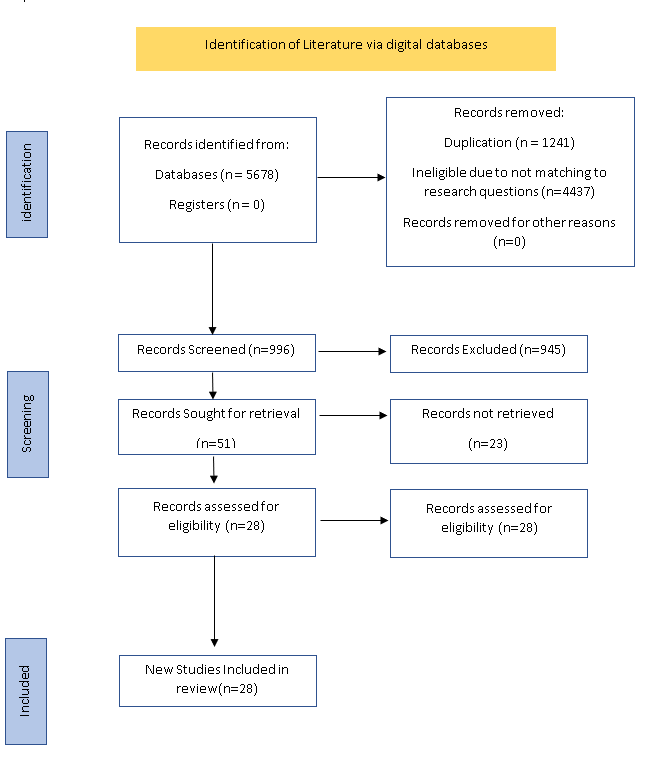
\includegraphics[width=\textwidth,keepaspectratio]{PRISMASummary.png}
  \caption{PRISMA Flowchart}\label{fig:prisma}
\end{figure*}


\afterpage{
  \clearpage
\begin{table*}[t]
  \centering
  \caption{PICO analysis for R1 papers MoA prediction from LINCS/CMap.}
  \begin{tabular}{p{3.1cm} p{4.8cm} p{5.1cm} p{3.3cm}}
    \toprule
    \textbf{Source} & \textbf{Problem} & \textbf{Intervention vs.\ Comparison (I/C)} & \textbf{Outcomes} \\
    \midrule
    \cite{subramanian2017next} (L1000 / CMap v2) &
    I\@:L1000 perturbational gene-expression profiles across many drugs/cell lines &
    Signature-similarity framework for drug, drug/MoA relationships;
    C\@: Prior CMap approaches / null connectivity &
    Improved coverage and scale; supports MoA inference and retrieval \\
    [0.35em]

    \cite{duan2016l1000cds2} (L1000CDS2)  &
    L1000 differential expression signatures (landmark/inferred genes) &
    I\@: Characteristic-Direction based signature search; 
    C\@: Other similarity/reversal metrics &
    Better reversal/connection retrieval; practical MoA/repurposing utility \\
    [0.35em]

    \cite{el2017integrative} (Integrative approach) &
    LINCS expression + auxiliary biomedical knowledge &
    I\@: Integrative similarity/knowledge fusion; 
    C\@: Expression-only similarity &
    Stronger MoA/indication signals via multimodal integration \\
    [0.35em]

    \cite{mcdermott2019deep} (DL benchmarks) &
    L1000 profiles for drug property / MoA categorization &
    I\@: MLPs (FF-ANN); 
    C\@: RF/SVM/logistic baselines &
    MLPs outperform classical ML\; interpretability trade-off noted \\
    [0.35em]

    \cite{liao2023open} (Open MoA) &
    Public MoA annotations + molecular/network priors &
    I\@: Network/topology-driven MoA inference; 
    C\@: Expression-only or shallow models &
    Competitive MoA accuracy with more interpretable, mechanism-grounded outputs \\
    [0.35em]

    \cite{lu2021drug} (WRFEN–XGBoost) &
    L1000 drug, cell line profiles with sparse coverage &
    I\@: Feature-engineered RF/ElasticNet + XGBoost; 
    C\@: vanilla RF/SVM baselines &
    Strong classical pipeline; competitive vs.\ deep models on some tasks \\
    [0.35em]

    \cite{pham2021deep} (DeepCE) &
    L1000 with drug structure features &
    I\@: Attention-based DL linking substructures to gene effects; 
    C\@: MLP/RF and non-attention models &
    Higher accuracy; interpretable substructure–gene attributions \\
    [0.35em]

    \cite{wu2022deep} (MultiDCP) &
    L1000 across diverse cell types / doses &
    I\@: Knowledge-aware Transformer for cross-cell generalization; 
    C\@: expression-only or non-attention DL &
    Better OOD prediction; sometimes surpassing noisy experimental baselines \\
    [0.35em]

    \cite{chow2022predicting} (Survey/context) &
    Pharmacogenomic prediction landscape incl.\ L1000 use-cases &
    I/C\@: Synthesis of attention/Transformer trends vs.\ prior methods &
    Frames accuracy, interpretability, scalability trade-offs \\
    \bottomrule
  \end{tabular}
\end{table*}

\begin{table*}[t]
  \centering
  \caption{PICO analysis for R2: data quality issues in LINCS L1000 and mitigation strategies.}
  \begin{tabular}{p{3.1cm} p{4.8cm} p{5.8cm} p{3.3cm}}
    \toprule
    \textbf{Source} & \textbf{Problem} & \textbf{Intervention vs.\ Comparison (I / C)} & \textbf{Outcomes} \\
    \midrule
    \cite{qiu2020bayesian} &
    L1000 bead deconvolution errors and peak-calling instability &
    I\@: GMM/AGMM and Bayesian deconvolution replacing $k$-means; C\@: original L1000 $k$-means / default pipeline &
    Lower deconvolution error; improved signature reliability and downstream accuracy \\[0.35em]

    \cite{subramanian2017next} &
    L1000 platform with 978 measured + $\sim$11k inferred genes; MODZ aggregation &
    I\@: Platform-level QC \& aggregation (e.g., MODZ); 
    C\@: naïve averaging / no QC &
    Scalable signatures; documents inferential noise sources to consider in modeling \\[0.35em]

    \cite{szalai2019signatures} &
    Replicate inconsistency; metadata/label noise in perturbational transcriptomics &
    I\@: Replicate-correlation filtering; robust losses/co-teaching framing; 
    C\@: unfiltered data / standard CE loss &
    Cleaner training sets; guidance on label-noise sensitivity and mitigation \\[0.35em]

    \cite{duan2016l1000cds2} &
    Noisy DE signatures reduce connectivity/reversal quality &
    I\@: Characteristic Direction (CD) signature generation; 
    C\@: fold-change / $t$-statistic signatures &
    Higher signal-to-noise; better reversal/connectivity retrieval \\[0.35em]

    \cite{pham2021deep} (DeepCE) &
    Noisy or low-quality replicates in L1000 training data &
    I\@: Model-guided data augmentation \& salvage of reliable replicates; 
    C\@: standard training without augmentation &
    Larger effective clean set; accuracy gains with interpretable attributions \\[0.35em]

    \cite{bang2024transfer} &
    Scarce clean labels; abundant unlabeled/noisy L1000 profiles &
    I\@: Self/semi-supervised pretraining then fine-tuning; 
    C\@: supervised from scratch &
    More robust representations; better generalization under noise \\[0.35em]

    \cite{mcdermott2019deep} &
    Benchmarks on L1000 for drug/MoA tasks, highlighting noise effects &
    I\@: MLPs with standard preprocessing; 
    C\@: RF/SVM/logistic baselines &
    DL $>$ classical but sensitive to data quality; motivates robust pipelines \\
    \bottomrule
  \end{tabular}
\end{table*}

\begin{table*}[t]
  \centering
  \caption{PICO analysis for R3: integrating external knowledge to improve performance and interpretability.}
  \begin{tabular}{p{3.1cm} p{4.8cm} p{5.8cm} p{3.3cm}}
    \toprule
    \textbf{Source} & \textbf{Population / Problem (P)} & \textbf{Intervention vs.\ Comparison (I / C)} & \textbf{Outcomes (O)} \\
    \midrule

    \cite{liu2015compound} &
    L1000 perturbational expression + drug chemical structure &
    I\@: Expression–structure fusion for signature/compound relationships; 
    C\@: expression-only similarity models &
    Stronger MoA/target signal and retrieval vs.\ expression-only \\[0.35em]

    \cite{stahlschmidt2022multimodal} &
    Multimodal biomedical learning settings (expression, chemistry, networks) &
    I\@: Early/intermediate/late fusion taxonomies (emphasis on intermediate); 
    C\@: single-modality pipelines &
    Guidance that intermediate fusion often outperforms simple early fusion \\[0.35em]

    \cite{elabd2024simple} &
    Cross-modal alignment for drug–gene/pathway effects; GO-informed designs &
    I\@: Cross-attention fusion and knowledge-infused architectures (e.g., GO hierarchy/DrugCell-style); 
    C\@: feature concatenation or black-box DL without priors &
    Better modality alignment and more interpretable, pathway-level attributions \\[0.35em]

    \cite{mcdermott2019deep} &
    L1000 expression with biological networks (e.g., PPI) &
    I\@: Graph CNNs leveraging network topology; 
    C\@: MLP/classical baselines without network priors &
    Pathway/module-aligned features; may need larger datasets to outperform MLPs \\[0.35em]

    \cite{samal2022opportunities} &
    Need for transparency in drug-response/MoA models &
    I\@: Intrinsically interpretable/knowledge-guided models vs.\ post-hoc XAI; 
    C\@: opaque black-box architectures &
    Mechanism-grounded “glass-box” explanations preferred over post-hoc attributions \\[0.35em]

    \cite{lu2021drug} &
    L1000 profiles with classical ML pipeline &
    I\@: WRFEN–XGBoost with feature selection (gene importance ranking); 
    C\@: opaque DL without clear attributions &
    Competitive accuracy; ranked gene lists provide direct interpretability \\[0.35em]

    \cite{ye2025knowledge} &
    Phenotype-based (expression) + target-based knowledge in one model &
    I\@: Knowledge-guided graph learning bridging phenotype and targets; 
    C\@: phenotype-only DL/ML &
    Improved performance and more auditable, target-centered rationales \\
    \bottomrule
  \end{tabular}
\end{table*}
\clearpage
}
\subsection{Synthesis of Results}
\textbf{R1: Techniques for Predicting Drug MoA and the Balance of Accuracy, Scalability, and Interpretability}
The literature reveals a clear usage of computational methods for MoA prediction, where a continuous search for higher accuracy is conducted while battling with the challenges of scalability and interoperability.
    \begin{itemize}
        \item \textbf{Early Approaches: Statistical Similarity and Classical Machine Learning:}
        \\
        Initially, the methods were based on the Connectivity Map hypothesis, using statistical methods to find drugs with similar gene expression signatures\cite{subramanian2017next,el2017integrative,liao2023open}. As data sets grew, the field adopted classical machine learning models. For instance, Random Forests were shown to be effective for predicting drug targets, particularly due to their inherent ability to handle the missing data that arises when not all drugs are tested in all cell lines\cite{mcdermott2019deep,subramanian2017next,duan2016l1000cds2}. Also methods like Support Vector Machines (SVMs) and regularised logistic regression were also used as strong baselines. While interpretable through feature importance scores, these models often struggled to capture complex, non-linear patterns in the high-dimensional gene expression space\cite{mcdermott2019deep}. For example, Lu et al. (2021) developed a hybrid WRFEN-XGBoost algorithm, demonstrating that highly optimized classical ML pipelines, which combine robust feature selection with powerful gradient boosting, remain a competitive approach for predicting drug sensitivity from L1000 profiles\cite{lu2021drug}
        \item \textbf{The Deep Learning Shift: From MLPs to GNNs:}
        \\
        The introduction of deep learning marked a huge performance leap. Simple fully connected feed-forward artificial neural networks (FF-ANNs), or multilayer perceptrons (MLPs), always outperformed classical ML baselines in predicting drug properties and therapeutic categories\cite{mcdermott2019deep}. The higher the accuracy, the lower the interpretability in these methods, as the models were treated largely as black boxes\cite{samal2022opportunities}. A huge leap from previous stages was the use of graph convolutional neural networks (GCNNs), which incorporate biological knowledge, such as a protein-protein interaction (PPI) network, directly into the model's structure. This constrains the model to learn features corresponding to biological pathways, offering a path back to interpretability.  Studies found that GCNNs can be highly performant but often require very large datasets to be effective, underperforming FF-ANNs on smaller corpora\cite{mcdermott2019deep}.
    
        \item \textbf{The Current Frontier: Attention Mechanisms and Transformers: }
        \\
         Today’s most advanced models in biology are inspired by tools originally built for understanding human language — specifically, attention mechanisms and transformer architectures. These models are incredibly powerful because they can uncover complex patterns and relationships in different types of data at the same time\cite{wu2022deep}.
    
        For example, a model called DeepCE uses a special attention technique to figure out how the tiny building blocks of a drug interact with specific genes. This helps predict how new, untested chemicals might affect gene activity — a big step forward for drug discovery\cite{pham2021deep}.
    
        Another model, MultiDCP, goes even further. It uses biological knowledge alongside transformer architecture to predict how cells will respond to drugs, even in completely new cell types. Remarkably, it can sometimes make predictions that are more reliable than actual experimental results, which are often noisy or inconsistent\cite{wu2022deep}.
    
        These models are pushing the limits of what’s possible in terms of accuracy and scale, but they also come with a trade-off: their inner workings are highly complex, making it difficult for researchers to explain or validate their predictions. Still, they represent an exciting leap forward in computational biology\cite{chow2022predicting}.
\end{itemize}



\textbf{R2: The Impact of Data Quality and Mitigation Strategies}
\\
The inconsistent or missing multifaceted noise that is inherent in the LINCS L1000 dataset affects the performance and the generalisability of predictive models hugely\cite{szalai2019signatures}. The literature describes both the sources of this noise and a range of strategies developed to address them.
\\
\\
\begin{itemize}
  \item \textbf{Sources of Noise}
    \begin{itemize}
            \item \textbf{Technical and Inferential Noise:}
            One of the main reasons for errors in the L1000 data comes from its technical process. The original method they used — a k-means algorithm for separating signal peaks — turned out to be unreliable, which led to inaccurate gene expression readings. To fix this, researchers have come up with better approaches, like Gaussian Mixture Models (GMM), Aggregate GMM (AGMM), and more recently, Bayesian models that are more stable and can deal better with uncertainty and outliers\cite{qiu2020bayesian}.
        
            Another big challenge is that the L1000 system only measures 978 landmark genes directly. The rest — about 11,000 genes — are generated using algorithms, not actually measured. This means that a large part of the dataset is based on predictions, which can be less reliable and adds another layer of noise\cite{subramanian2017next,mcdermott2019deep}.
            \item \textbf{Metadata Inconsistency and Label Noise: }
            The annotations that are associated with the data shows huge errors and inconsistencies in the LINCS L1000 dataset. This includes missing MoA labels, inconsistent drug identifiers, and heterogeneity in how information is recorded. These issues translate directly into label noise for supervised models, that can really damage the model more than the noisy features\cite{szalai2019signatures}. 
            \end{itemize}
        \item \textbf{Mitigation Strategies:}
    
            \begin{itemize}
            \item \textbf{Data-Centric Approaches:}
            
            The methods that is trying to be implemented aim to improve data quality before the modelling stage. One of the best practices, when it comes to these type of moments, is the use of superior signature generation methods like the Characteristic Direction (CD), which has been shown to significantly improve the signal-to-noise ratio over default methods\cite{duan2016l1000cds2}. To filter out unreliable experiments, another common technique used is data cleaning based on replicate correlation\cite{szalai2019signatures}. If a more advanced strategy is considered, then the data augmentation strategy in DeepCE can be mentioned. It uses a trained model to identify and salvage reliable bio-replicated data from experiments initially flagged as noisy, thereby increasing the size of the high-quality training set\cite{pham2021deep}.
                \\
            \item \textbf{Model-Centric Approaches:} 
            The main strategy is to build models that are inherently robust to noise. This is a great research area, with several techniques being applied. 
            \begin{itemize}
            \item \textbf{Robust Loss Functions:} To prevent models from overfitting to label noise, we can use loss functions like Mean Absolute Error (MAE) or generalized cross-entropy, which are bounded and are less sensitive to confidently wrong (e.g., mislabeled) examples\cite{szalai2019signatures}.
            \item \textbf{Robust Training Procedures:} To prevent the memorization of noisy labels, techniques like co-teaching can be used, where two networks are trained in parallel and teach each other using only their most confident (lowest-loss) predictions\cite{szalai2019signatures}. Another effective strategy is curriculum training, where a model is first trained on easy/clean examples before being exposed to harder/noisier data\cite{pham2021deep}.
            \item \textbf{Self-Supervised and Semi-Supervised Learning:} These paradigms are powerful for leveraging the vast amount of unlabelled or noisy labelled data. Models can be pre-trained on a task that doesn't require clean labels (e.g., a denoising autoencoder that learns to reconstruct a clean profile from a corrupted one) to learn robust representations of the data structure. This pre-trained model can then be fine-tuned on a smaller, cleaner dataset for the final prediction task\cite{bang2024transfer}.
    \end{itemize}
  \end{itemize}
\end{itemize}
\textbf{R3: Integration of External Knowledge and Impact on Interpretability}
The most advanced frameworks recognize that gene expression is only one piece of the puzzle and actively integrate external knowledge to build more powerful models.
\\
\begin{itemize}
    \item \textbf{Rationale and Fusion Architectures:} The primary motivation is to combine complementary information: a drug's chemical structure governs over the fact of its physical properties and target areas, while biological networks (e.g., PPIs, Gene Ontology) provide the cellular context in which the drug acts\cite{liu2015compound}. Flexible architectures are provided by deep learning for multimodal fusion. While simple early fusion (combining raw features) is possible, intermediate fusion is the more dominant strategy. This involves using a lot of separate branches of networks before fusing them in a deep layer in order to learn high-level representations of each modality\cite{stahlschmidt2022multimodal}. Recent models use complex fusion mechanism like cross-attention, which allows the model to learn alignments between modalities dynamically, such as which part of a drug's structure is most relevant to which gene pathways\cite{elabd2024simple}.
    \item \textbf{Knowledge-Infused Architectures and Intrinsic Interpretability:} A more profound form of integration is knowledge infusion, where the architecture is defined by biological priors. The use of GCNNs operating on a fixed PPI network is a prime example, which forces the model to learn features that correspond to network modules\cite{mcdermott2019deep}. The DrugCell model represents the highest point of this approach\cite{elabd2024simple}.  Its architecture is a direct implementation of the Gene Ontology (GO) hierarchy.  Each neuron corresponds to a specific biological subsystem, and connections mirror the GO structure. The activation of a neuron, therefore, has a direct biological interpretation: the predicted activity of that subsystem in response to the drug\cite{samal2022opportunities}.
    \item \textbf{Impact on Interpretability:} th eshift twoards deep learning gave us the black box problem.IN this cas the models precitions are hard to understand and explain. Some models provide interpretability intrinsically through their architecture rather than through post-hoc XAI techniques. The WRFEN-XGBoost model, for instance, yields a ranked list of the most influential genes used for its predictions (Lu et al., 2021)\cite{lu2021drug}. Integrating external knowledge is a primary driver for enhancing model interpretability. While post-hoc methods can be applied to any trained model to assign feature importance, knowledge-infused models are interpretable by design\cite{samal2022opportunities}. Instead of requiring a secondary method to explain a prediction, one can directly inspect the model's internal state to understand its mechanistic hypothesis, moving from opaque  \enquote{black boxes} to transparent \enquote{glass boxes}.
\end{itemize}

\section{Discussion}
\subsection{Summary of Evidence}

    This systematic review confirms that the prediction of drug MoA from LINCS L1000 data is a mature yet rapidly evolving field. The pathway of computational methods shows a clear and logical progression from simple statistical matching to classical machine learning, and now to increasingly complicated deep learning architectures (R1). This evolution has been driven by the quest for greater predictive accuracy, with FF-ANNs, GCNNs, and now Transformer-based models setting new performance benchmarks\cite{mcdermott2019deep}.
    However, high performance is contingent on addressing the significant data quality challenges inherent to the LINCS L1000 platform (R2). The challenge is not only one of quality but also of scale and accessibility; in response, the community has developed powerful data exploration platforms like the L1000FWD web server, which provides an interactive interface for visualizing the entire signature landscape (Wang et al., 2018)\cite{wang2018l1000fwd}.The literature provides a detailed anatomy of these noise sources—from technical assay artifacts to metadata inconsistencies—and a corresponding collection of mitigation strategies\cite{qiu2020bayesian}. A key shift is the move from simply filtering the noise to developing robust models that can learn effectively in its presence, using techniques like noise-robust loss functions, curriculum learning, and self-supervision.
    The most advanced frameworks achieve superior performance and interpretability by combining external knowledge (R3). Integrating transcriptomic data with drug chemical structures and biological networks provides complementary information that grounds models in mechanistic reality~\cite{wang2016drug}. The development of knowledge-infused architectures, where the model's structure mirrors biological hierarchies like the Gene Ontology, represents a paradigm shift towards models that are interpretable by design, showing transparency into the decision-making process, which is vital in a medical perspective~\cite{samal2022opportunities}.

\subsection{Limitations and Future Directions}

Despite the progress, several critical challenges and limitations persist, defining the frontier for future research.
    \begin{itemize}
        \item \textbf{The Validation Gap in Interpretability: } The most significant gap identified in this review is the lack of rigorous, quantitative validation for model interpretations.Most studies still rely on qualitative, anecdotal validation by searching the literature for confirmation of a model's top-ranked genes or pathways\cite{samal2022opportunities}. This is susceptible to confirmation bias and fails to validate novel discoveries. The development of scalable, quantitative validation frameworks, such as the hypothesis-driven Global Importance Analysis (GIA) or in-silico perturbation experiments, is a critical and unmet need. Without robust validation, the `explanations' from XAI methods remain unproven hypotheses.
        \item \textbf{Generalization to Unseen Contexts:}Many models exhibit a significant drop in performance when tested on data from unseen subjects, tissues, or populations, highlighting a major challenge in out-of-distribution generalization\cite{mcdermott2019deep}. This severely limits the clinical translatability of these models. Future work must focus on developing architectures and training schemes (e.g., leveraging domain adaptation) that are explicitly designed and validated for their ability to generalize across diverse biological contexts.
        \item \textbf{Handling Structured, Real-World Noise:} While many noise-robust learning techniques exist, most are benchmarked on synthetic, uniform noise models. The noise in LINCS is complex and structured. There is a clear need for methods tailored to this specific noise profile, moving beyond generic solutions to address the unique combination of technical, inferential, and annotation-based errors.
    \end{itemize}

\subsection{Conclusion}
The use of interpretable deep learning for MoA prediction from noisy LINCS L1000 data is a vibrant and impactful field. The community has made substantial progress in developing powerful predictive models, identifying and mitigating data quality issues, and integrating multimodal knowledge to create more interpretable systems. However, for these powerful tools to translate into trusted instruments for clinical decision-making and scientific discovery, the field must now pivot to address the grand challenges of quantitative validation and robust generalization. The journey from black box to glass box is well underway, but the path to a truly trustworthy and validated AI for drug discovery requires a concerted focus on these remaining frontiers.

\section{Other information}

\textbf{Funding: }This research received no specific grant from any funding agency in the public, commercial, or not-for-profit sectors.

\textbf{Author Contributions: }N.H. conceptualized the study, conducted the literature search, screened the articles, and wrote the original draft. S.V. supervised the project, provided critical feedback, and reviewed and edited the manuscript. Both authors have read and agreed to the published version of the manuscript.

% \textbf{Conflicts of Interest:}The authors declare no conflict of interest.

\bibliographystyle{unsrtnat}
\nocite{*}
\bibliography{references}
\end{document}